\documentclass{beamer}
\usepackage{graphicx}
\graphicspath{ {./images/} }
\usepackage[rightcaption]{sidecap}

\usefonttheme[onlymath]{serif}
%\definecolor{LHCblue}{RGB}{4, 114, 255}
%\usecolortheme[named=LHCblue]{structure}
\usepackage[bars]{beamerthemetree} % Beamer theme v 2.2
\usepackage{multicol}
\usepackage{lmodern}
\usepackage{lipsum}
\usepackage{marvosym}

\usetheme{Berlin}
\setbeamertemplate{blocks}[default]
\useinnertheme{circles} % change the bullets' shape
\setbeamertemplate{caption}[numbered] % number the figures
\usepackage[textfont={scriptsize}]{caption}
\usepackage{tikz} % for checkmarks

\setbeamertemplate{footline}{\begin{tikzpicture}
    \node [inner sep=0pt, anchor=east] (0,0) {
\includegraphics[width=\paperwidth,height=0.7cm]{12_espa}};
%    \node [inner sep=0pt, anchor=east] at (-2ex,-3ex) {\insertframenumber{} / %\inserttotalframenumber};
\end{tikzpicture}}

\title{Open tools and methodology for the development of a web-based transportation platform}
%\author{Babalis B*, Ballis A., Koukoutsis E.}
%\institute{National Technical University of Athens}
%\date{2021}

\author[Babalis B., Ballis A., Koukoutsis E.] % (optional, for multiple authors)
{Babalis B.\inst{1} \and Ballis A.\inst{2} \and Koukoutsis E.\inst{1}}

\institute[National Technical University of Athens] % (optional)
{
  \inst{1}%
  School of Electrical and Computer Engineering\\
  National Technical University of Athens
  \and
  \inst{2}%
  School of Civil Engineering\\
  National Technical University of Athens
}

\date[CES 2021] % (optional)
{Circular Economy and Sustainability, July 2021}

\logo{
\includegraphics[height=1cm]{09_pyrforos_bw}}

\begin{document}

\frame{\titlepage}

\begin{frame}
	\frametitle{Table of Contents}
	\tableofcontents
\end{frame}

\section{Introduction}
    \begin{frame}
    \frametitle{Introduction}
    A transportation platform aim to deliver the supply chain solutions required for excellence in transportation sourcing, execution and management.\\
    Usually transportation platforms offer functionality based on:
    \begin{itemize}
    	\item Proprietary GIS systems.
    	\item Proprietary updates on network and data.
    	\item External, proprietary web applications.
    \end{itemize}
    \pause
    \checkmark As a result, such platforms heavily depend on their proprietary software.
    \end{frame}
    
    \begin{frame}
    \frametitle{Alternative approach}
    
    An alternative approach on building a web-based transportation platform is presented.
    \begin{block}{Alternative Approach}
    Platform based exclusively on free/open source data and tools.
	\end{block}

    \pause
    \begin{itemize}
        \item Open Data
        \item Open source tools for building the platform
        \item Open Maps
    \end{itemize}
    \end{frame}
    
    \begin{frame}
    \frametitle{Why open tools?}
    Why a platform based on open tools?
    
    \begin{itemize}
        \item Ensure sustainability of the system.
        \item Maintained by the community - no dependencies on proprietary tools.
        \item Data checked and maintained by community.
    \end{itemize}
    \end{frame}

\section{Architecture and Design}
    \begin{frame}
    \frametitle{Basic Platform Components}
    Basic blocks for building a web transportation platform:
    \begin{enumerate}
        \item Maps and geospatial data visualization tools.
        \item Data and tools for data selection and process.
        \item Set of functionalities offered through a web interface.
    \end{enumerate}
    
	\end{frame}
	
	\begin{frame}
    \frametitle{Abstract Methodology}
    For the alternative platform to be developed the following steps applied:
    
    \begin{itemize}
        \item Maps collected and integrated to the platform.
        \item Data collected from various sources.
        \item Data organized and integrated to the platform.
        \item Data visualizations computed and offered (through charts/pies and maps).
        \item Extra functionalities developed combining the data collected with geospatial information.
    \end{itemize}
    
    \end{frame}
    
    \begin{frame}
    \frametitle{Conceptual Architecture of the Platform}
    \begin{figure}[h]
    \centering
    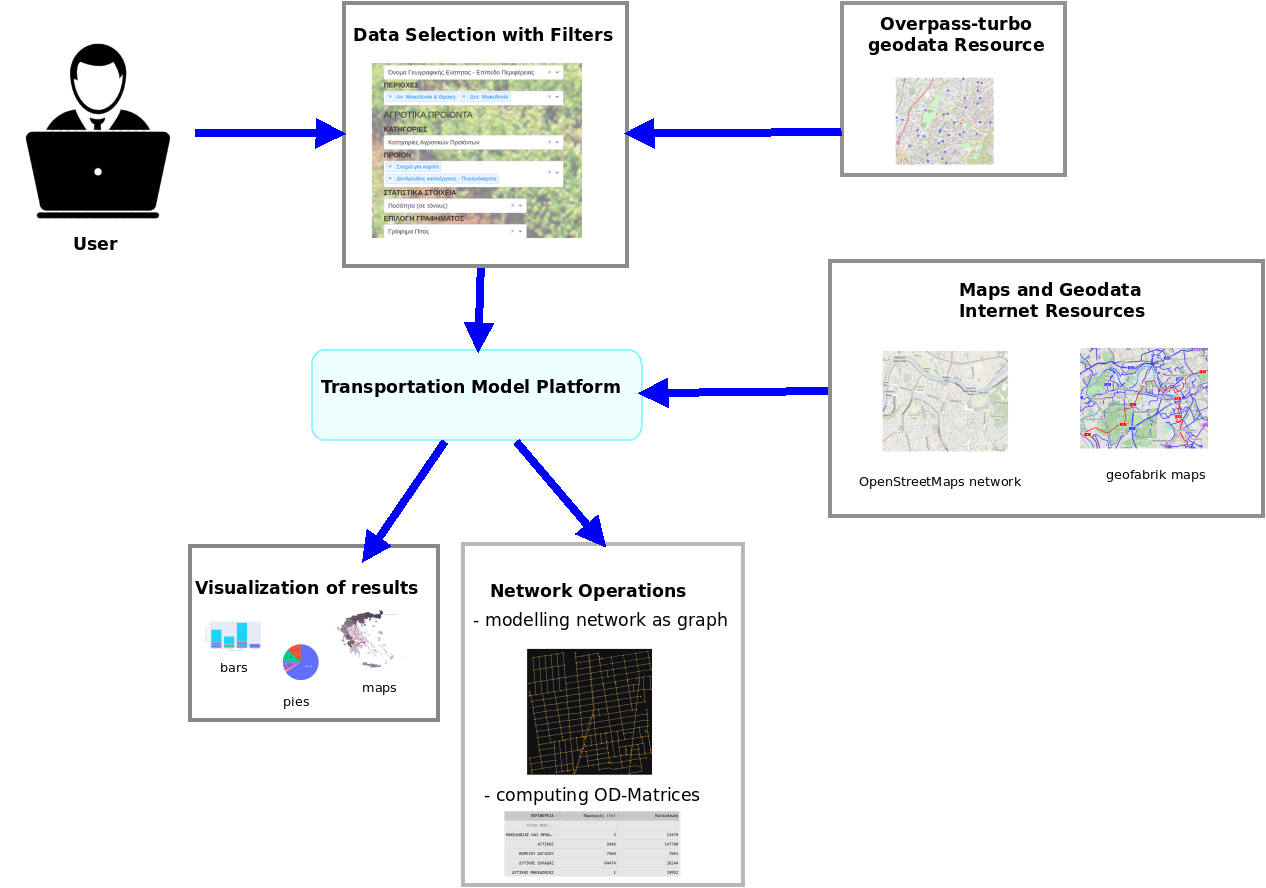
\includegraphics[width=8cm, height=5cm]{10_conceptual-architecture}
    \caption{Conceptual Architecture of the Platform.}
    \label{fig:arch}
    \end{figure}
    \end{frame}
    
   \section{Methodology}
    \begin{frame}
    \frametitle{Maps}
    The maps selected for the platform are the OpenStreetMaps (OSM).
    OSM is a collaborative project that creates a free, editable map of the world.
    
    \begin{block}{OpenStreetMaps}
		\begin{itemize}
        	\item It covers the world.
        	\item It is supported by OpenStreetMap Foundation (non-profit organization).
        	\item Open Database License (ODbL)
    	\end{itemize}
	\end{block}
    
    \end{frame}
    
    \begin{frame}
    \frametitle{Platform Data}
    
    \begin{itemize}
        \item Data has been collected from many, different sources (elstat, eurostat, et al)
        \item Data has been normalized and filters may be applied to create a custom configuration.
    \end{itemize}
    
    \begin{figure}[h]
    \centering
    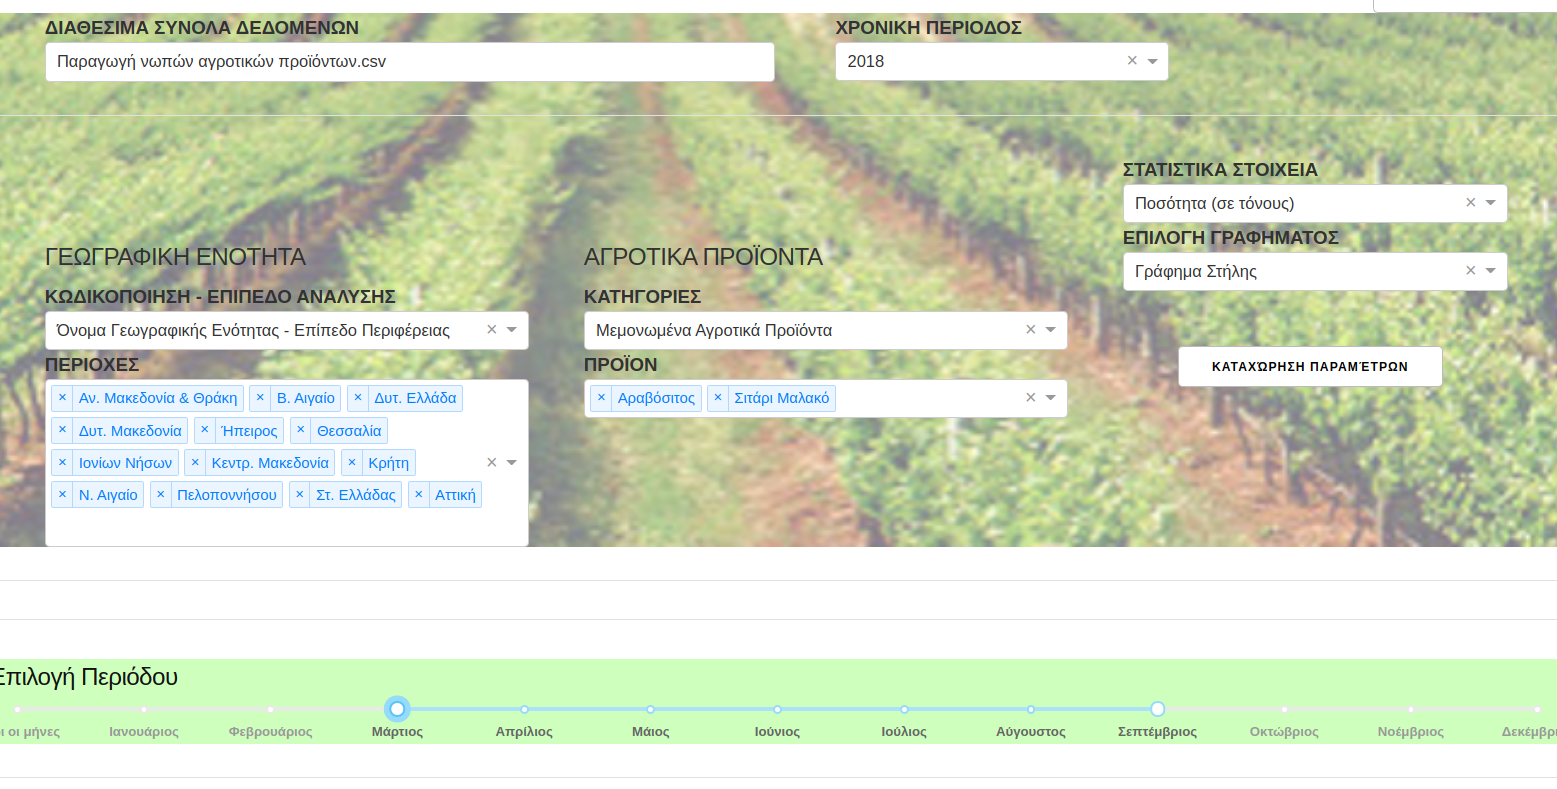
\includegraphics[width=7cm, height=3cm]{1_platform_filters}
    \caption{Filters applied to data available.}
    \label{fig:filters1}
    \end{figure}
    
    \end{frame}
    
    \begin{frame}
    \frametitle{Data Visualizations}
    
	    \begin{exampleblock}{Visualizing data}
	    Data selection is visualized through tables, charts, pies and choropleths.
		\end{exampleblock}
		
	%	\centering
	%        \begin{tabular}{c}
	%        example1\\
	%        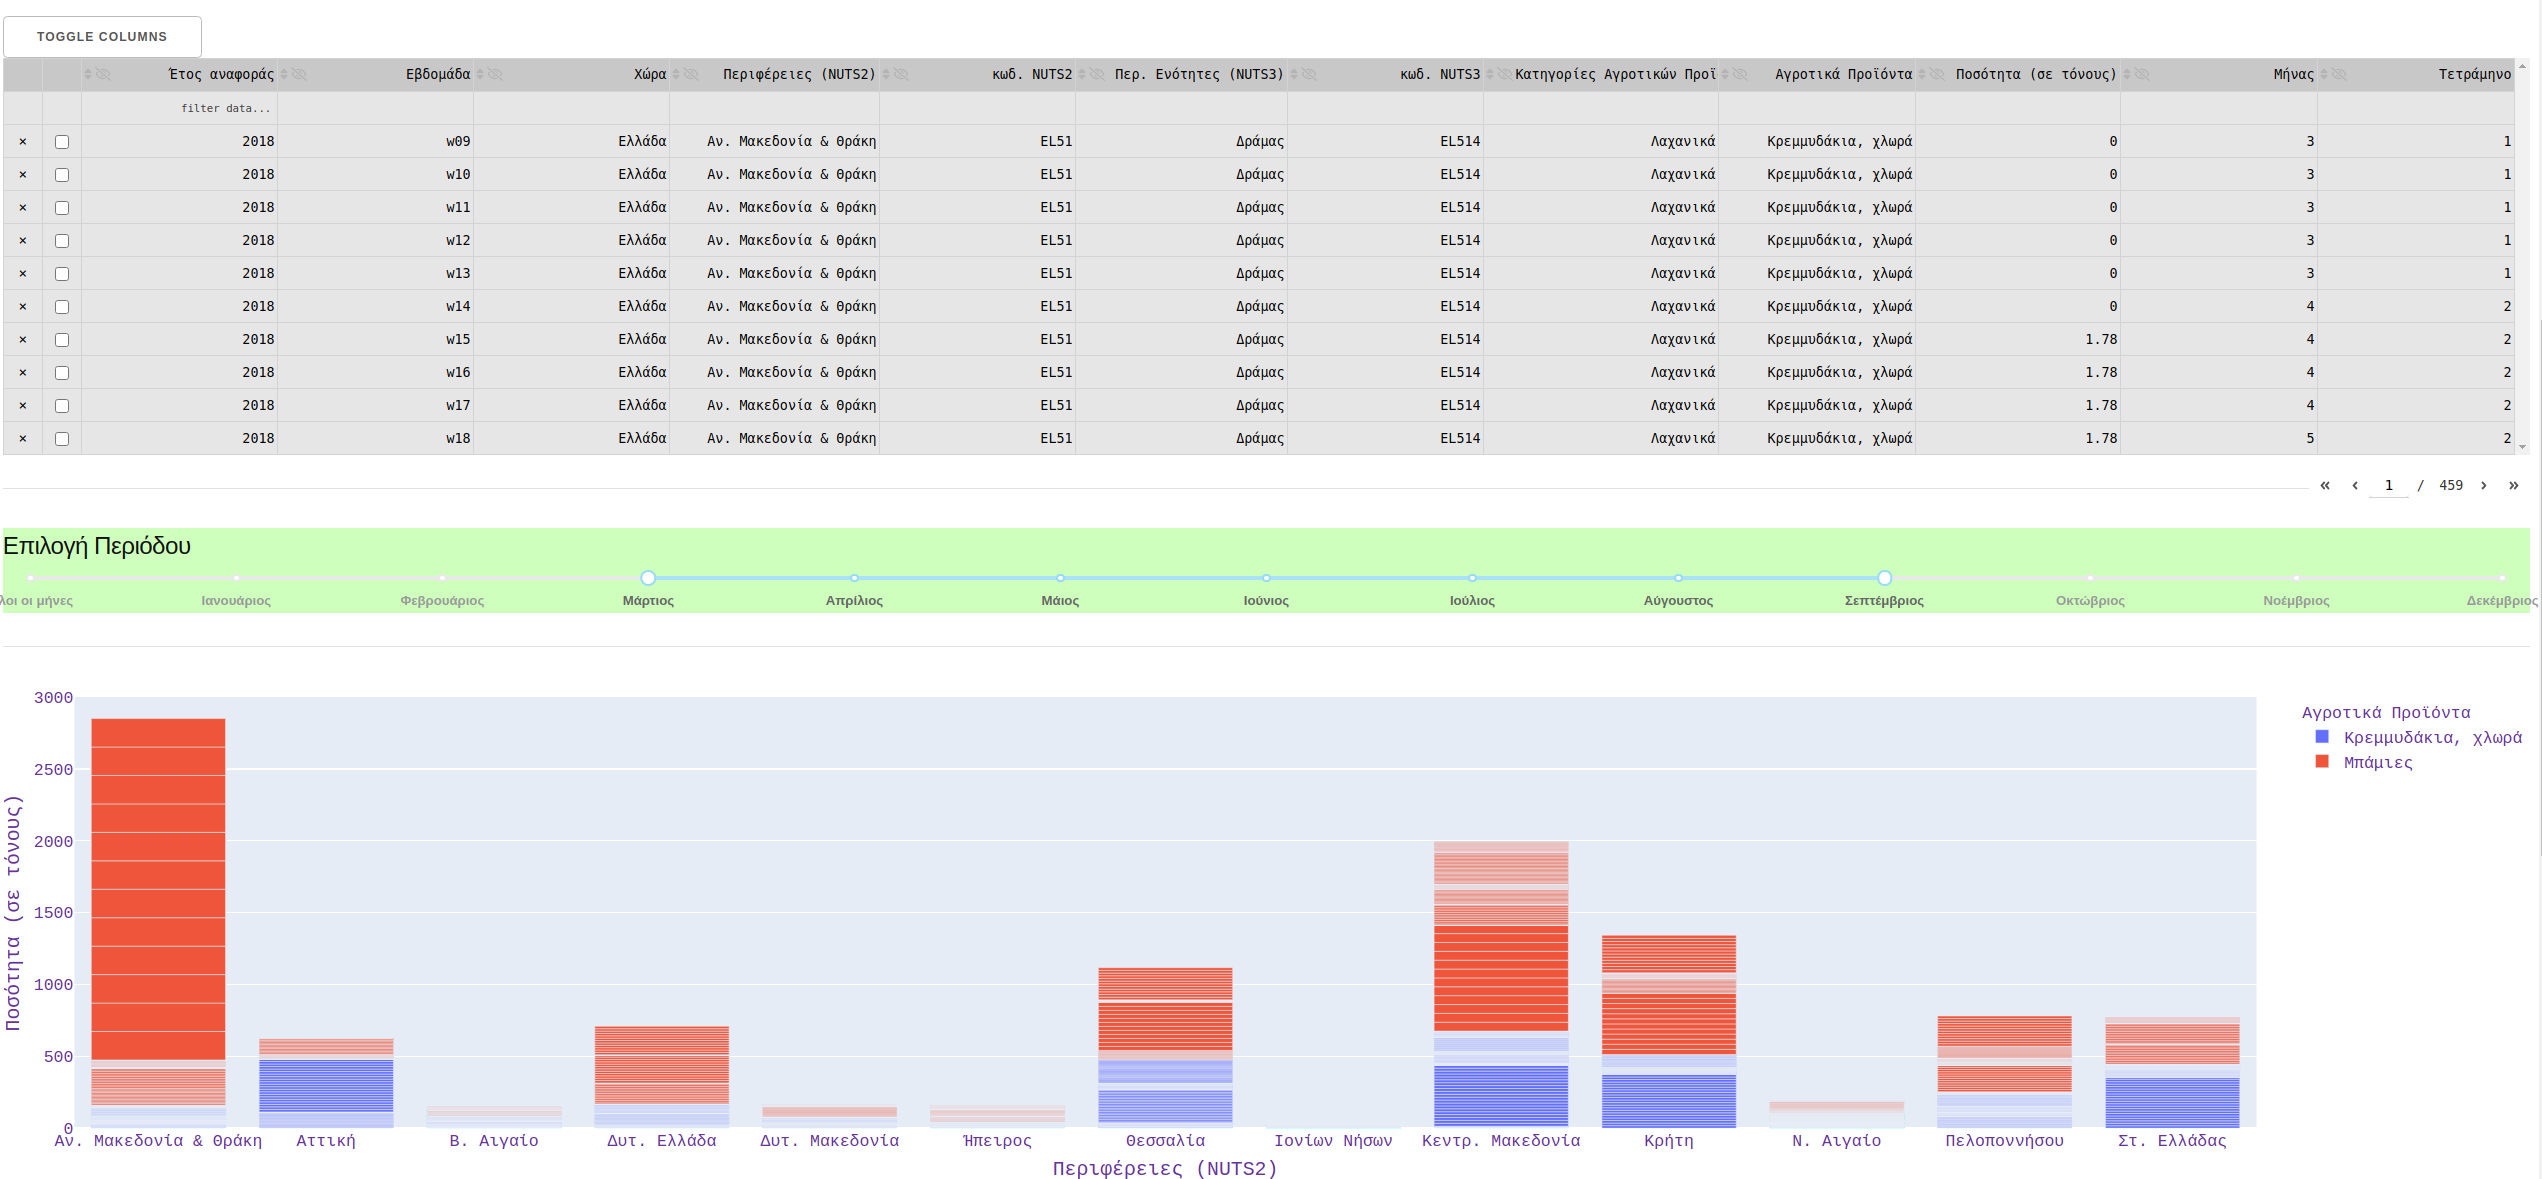
\includegraphics[width=3cm]{02_table_chart}
	%      \end{tabular}
	%
	%      \vspace{0.01em}
	%        \begin{tabular}{cc}
	%        example2  & example3 \\
	%        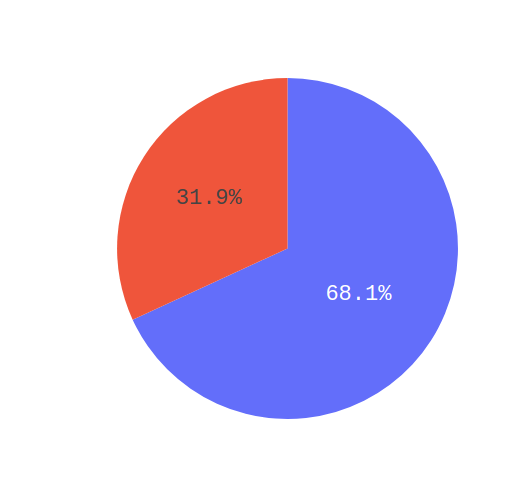
\includegraphics[width=3cm]{03_pie}
	%         &
	%         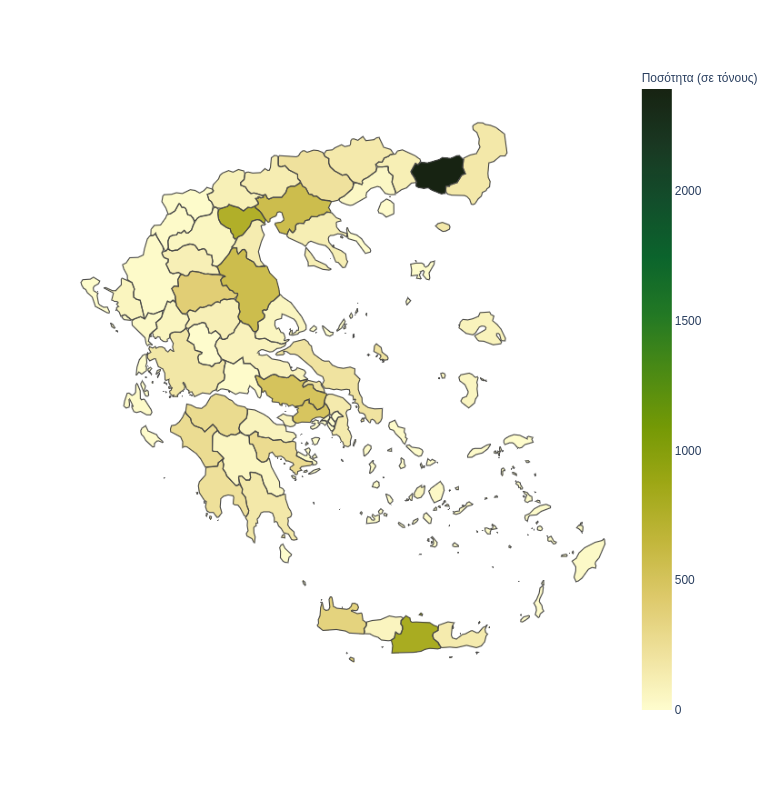
\includegraphics[width=3cm]{04_choropleth}
	%         \end{tabular}
		\begin{figure}[h]
		\begin{columns}[t]
			\column{.5\textwidth}
				\centering
				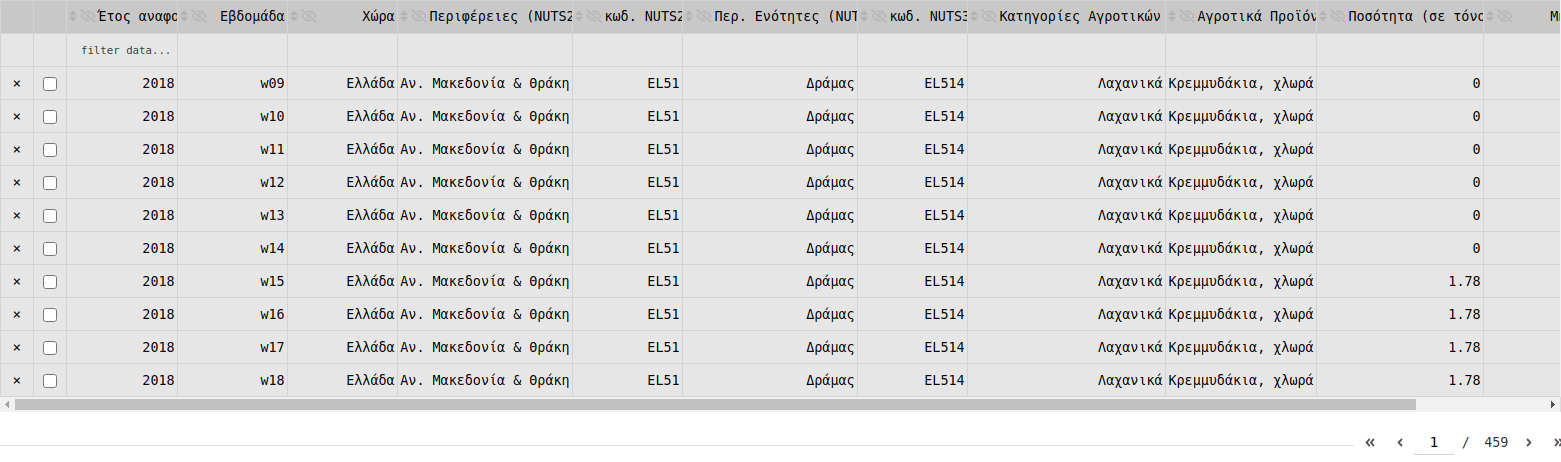
\includegraphics[width=5cm,height=2cm]{05_table}\\
				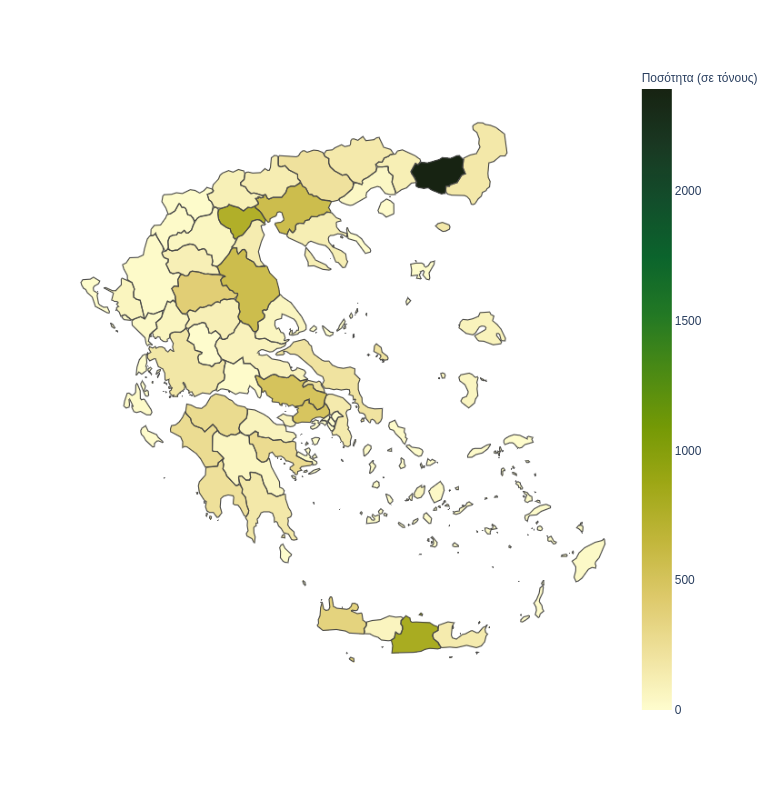
\includegraphics[width=3cm,height=2cm]{04_choropleth}
			\column{.5\textwidth}
				\centering
				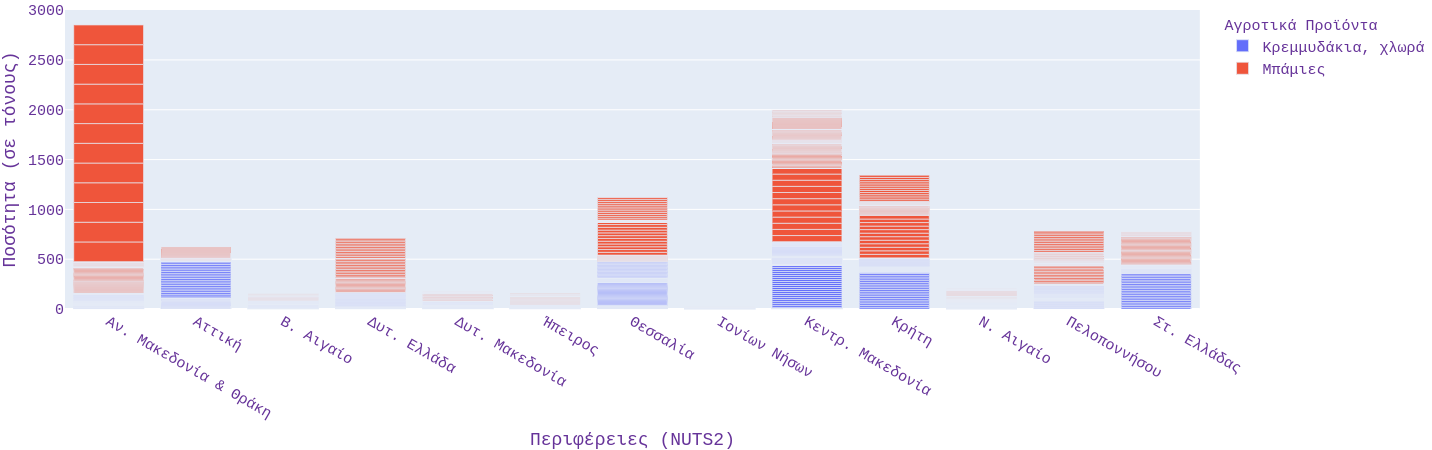
\includegraphics[width=5cm,height=2cm]{06_chart}\\
				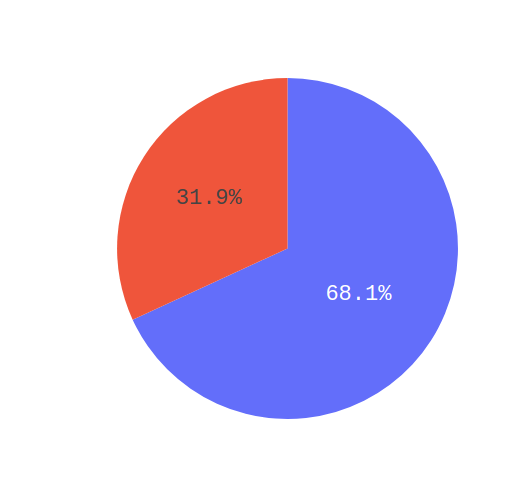
\includegraphics[width=2cm,height=2cm]{03_pie}
			\end{columns}
			\caption{Data visualization.}
			\label{fig:visuals}
	    \end{figure} 
    \end{frame}
    
    \begin{frame}
    \frametitle{Applications on selected data}
    By selecting a custom data sub-set the user may further use the platform for valuable insights.
    
    \begin{exampleblock}{Four Step Model app}
	    The user may execute a four-step-model on the selected data and get the results.
	\end{exampleblock}
	
	\begin{figure}[h]
    \centering
    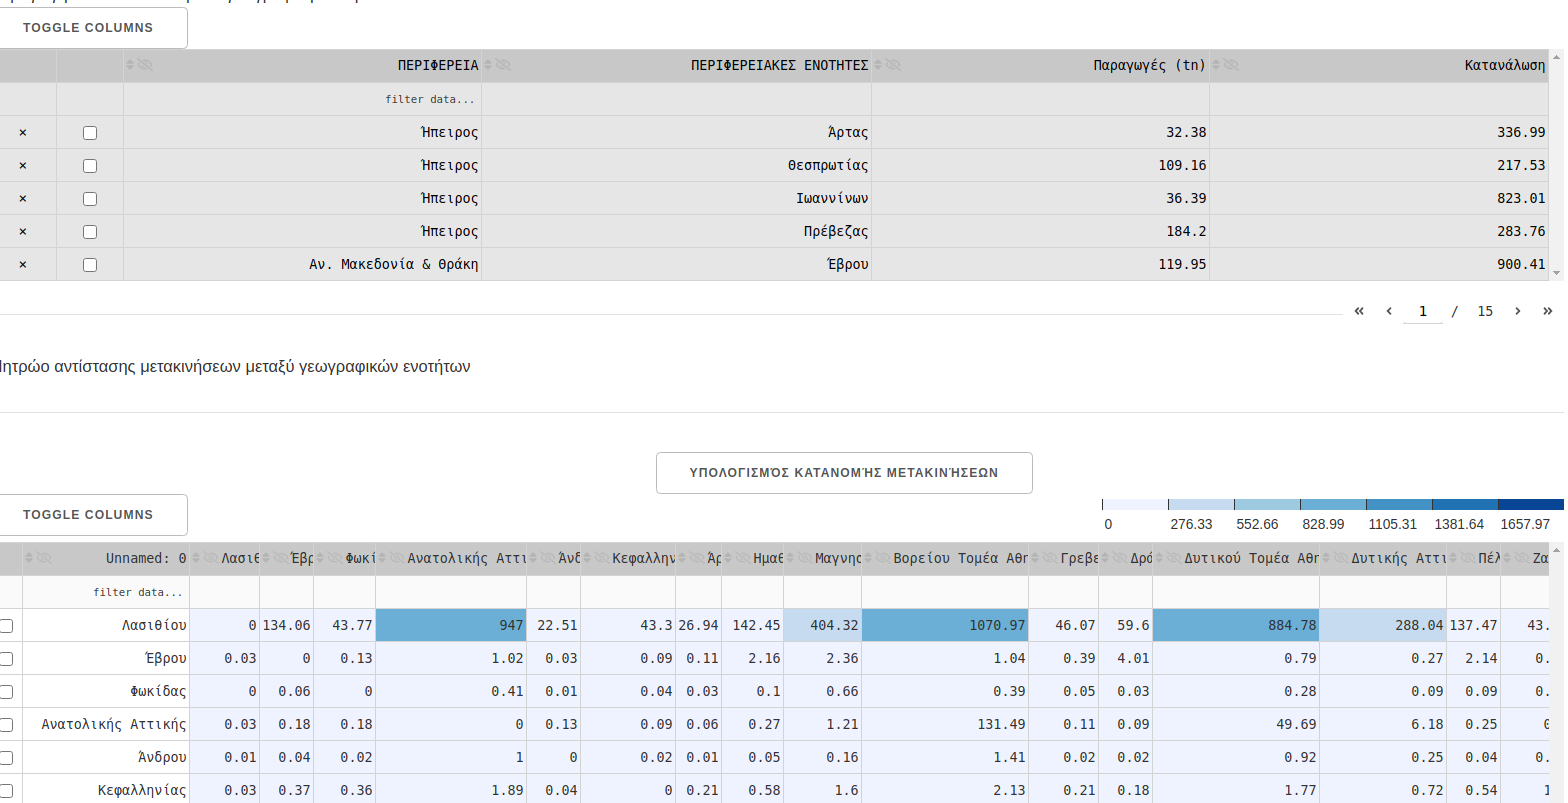
\includegraphics[width=8cm, height=3cm]{08_4sm}
    \caption{Four Step Model Execution based on user data selection.}
    \label{fig:4sm}
    \end{figure}
    
    \end{frame}

\section{Results}

	\begin{frame}
    \frametitle{Conclusions - Added value}
    Platform created as Proof of Concept.
    \begin{itemize}
        \item A web-based transportation platform can be built solely on open tools and data.
        \item Such a platform offers functionality and apps restricted only by its community.
        \item No proprietary software ensures sustainability of such a project.
    \end{itemize}
    
    \end{frame}
    
    \begin{frame}
    \frametitle{Restrictions - Future Work}
    \begin{itemize}
        \item Such a platform is heavily-bound to its users and the community.
        \item It can develop only so much as its users are interested to.
        \item Challenge: Platform integration to open geodata ecosystem.
    \end{itemize}
    
    \end{frame}

	
\end{document}